\chapter{Selective sweeps on different pigmentation genes mediate convergent evolution of island melanism in two incipient bird species} \label{chapter3}

\textit{Content of this chapter was published in PLoS Genetics (2022) under the title ``Selective sweeps on different pigmentation genes mediate convergent evolution of island melanism in two incipient bird species" by Leonardo Campagna, Ziyi Mo, Adam Siepel and J. Albert C. Uy. L.C. conceptualized the study, curated data, performed formal analyses, developed methodology and wrote the manuscript. Z.M. characterized selective sweeps in the bird populations using the SIA method, developed methodology and edited the manuscript. A.S. developed methodology and edited the manuscript. J.A.C.U. conceptualized the study, curated data, performed formal analyses, developed methodology and wrote the manuscript.}

\section{Abstract}

Insular organisms often evolve predictable phenotypes, like flightlessness, extreme body sizes, or increased melanin deposition. The evolutionary forces and molecular targets mediating these patterns remain mostly unknown. Here we study the Chestnut-bellied Monarch (\textit{Monarcha castaneiventris}) from the Solomon Islands, a complex of closely related subspecies in the early stages of speciation. On the large island of Makira \textit{M. c. megarhynchus} has a chestnut belly, whereas on the small satellite islands of Ugi, and \ac{SA/SC} \textit{M. c. ugiensis} is entirely iridescent blue-black (i.e., melanic). Melanism has likely evolved twice, as the Ugi and \ac{SA/SC} populations were established independently. To investigate the genetic basis of melanism on each island we generated whole genome sequence data from all three populations. Non-synonymous mutations at the \textit{MC1R} pigmentation gene are associated with melanism on \ac{SA/SC}, while \textit{ASIP}, an antagonistic ligand of \textit{MC1R}, is associated with melanism on Ugi. Both genes show evidence of selective sweeps in traditional summary statistics and statistics derived from the \acf{ARG}. Using the \ac{ARG} in combination with machine learning, we inferred selection strength, timing of onset and allele frequency trajectories. \textit{MC1R} shows evidence of a recent, strong, soft selective sweep. The region including \textit{ASIP} shows more complex signatures; however, we find evidence for sweeps in mutations near \textit{ASIP}, which are comparatively older than those on \textit{MC1R} and have been under relatively strong selection. Overall, our study shows convergent melanism results from selective sweeps at independent molecular targets, evolving in taxa where coloration likely mediates reproductive isolation with the neighboring chestnut-bellied subspecies.

\section{Introduction}
The extent to which evolutionary change can be predicted has been a longstanding matter of debate in evolutionary biology (\cite{gould1989wonderful,blount2018contingency,grant2002unpredictable}). Instances of convergent evolution support the argument that evolutionary change can be deterministic, yet stochastic historical events can lead to divergent outcomes from recently split taxa. A better understanding of the eco-evolutionary forces and genetic mechanisms behind evolutionary changes will shed light on the conditions under which deterministic or stochastic outcomes can occur. Some examples of convergent evolution occurred deep in the tree of life, like the independent origins of wings in birds, bats and insects (\cite{blount2018contingency}), while other cases represent more recent (and potentially ongoing) phenomena like the repeated radiations of ecomorphs in Caribbean lizards (\cite{mahler2013exceptional}), the loss of flight associated to insularity in insects and birds (\cite{roff1994evolution,wright2016predictable}) or the evolution of island melanism (\cite{mundy2005window}). These recent classic examples of phenotypic convergence can be leveraged to study the evolutionary forces and molecular mechanisms behind phenotypic change. Here we focus on island melanism in birds, a phenotype that involves the increased deposition of eumelanin, which leads to entirely black plumage coloration (\cite{theron2001molecular,uy2016mutations,walsh2021patterns}).

The Chestnut-bellied Monarch (\textit{Monarcha castaneiventris}) from the Solomon Islands represents a complex of closely related subspecies which are in the early stages of speciation and vary in plumage color, song, and body size (\cite{mayr1999systematics,mayr2001birds,uy2009plumage}). One of these subspecies, \textit{M. c. ugiensis}, has entirely iridescent blue-black plumage, and is found on the small satellite islands to the north and southeast of the larger island of Makira (Fig. \ref{fig:mon-F1}A). In contrast, the endemic subspecies on Makira is \textit{M. c. megarhynchus} and has a chestnut belly and iridescent blue-black upper parts. Phylogenetic analyses using reduced-representation genomic data show that \textit{M. c. ugiensis} individuals from the satellite islands of Ugi, and \acf{SA/SC} are independently derived from the chestnut-bellied Makira population, suggesting that \textit{M. c. ugiensis} is polyphyletic and melanism has evolved repeatedly and convergently (\cite{cooper2017genomic}). A candidate gene study suggested that the molecular basis of increased melanin deposition differs between the Ugi and \ac{SA/SC} populations (\cite{uy2016mutations}). Melanism on each of the satellite islands is associated with mutations that affect the coding sequence of the \textit{MC1R}/\textit{ASIP} receptor and ligand pair, two molecules that regulate the balance between the production of eumelanin (a pigment conferring black/gray coloration) and pheomelanin (a pigment which leads to brown/yellow coloration). While the melanic individuals from \ac{SA/SC} carry a derived non-synonymous mutation on the \textit{MC1R} receptor, their counterparts from Ugi possess a non-synonymous mutation on the \textit{ASIP} ligand, and heterozygotes at either mutation display an intermediate coloration phenotype (Fig. \ref{fig:mon-F1}B; \cite{uy2016mutations}). Finally, it is likely that changes in plumage color mediated by these mutations generate prezygotic reproductive isolation between the melanic populations on the satellite islands and the chestnut-bellied population on nearby Makira, as territorial males discriminate individuals by their phenotype, and respond predominantly to simulated territorial intrusions of males with the local plumage (and song) traits (\cite{uy2009difference,uy2013variation}). Convergent melanism, therefore, may result in repeated speciation between the chestnut-bellied population of Makira, and each of the two melanic populations of Ugi and \ac{SA/SC}.

\begin{figure}
    \centering
    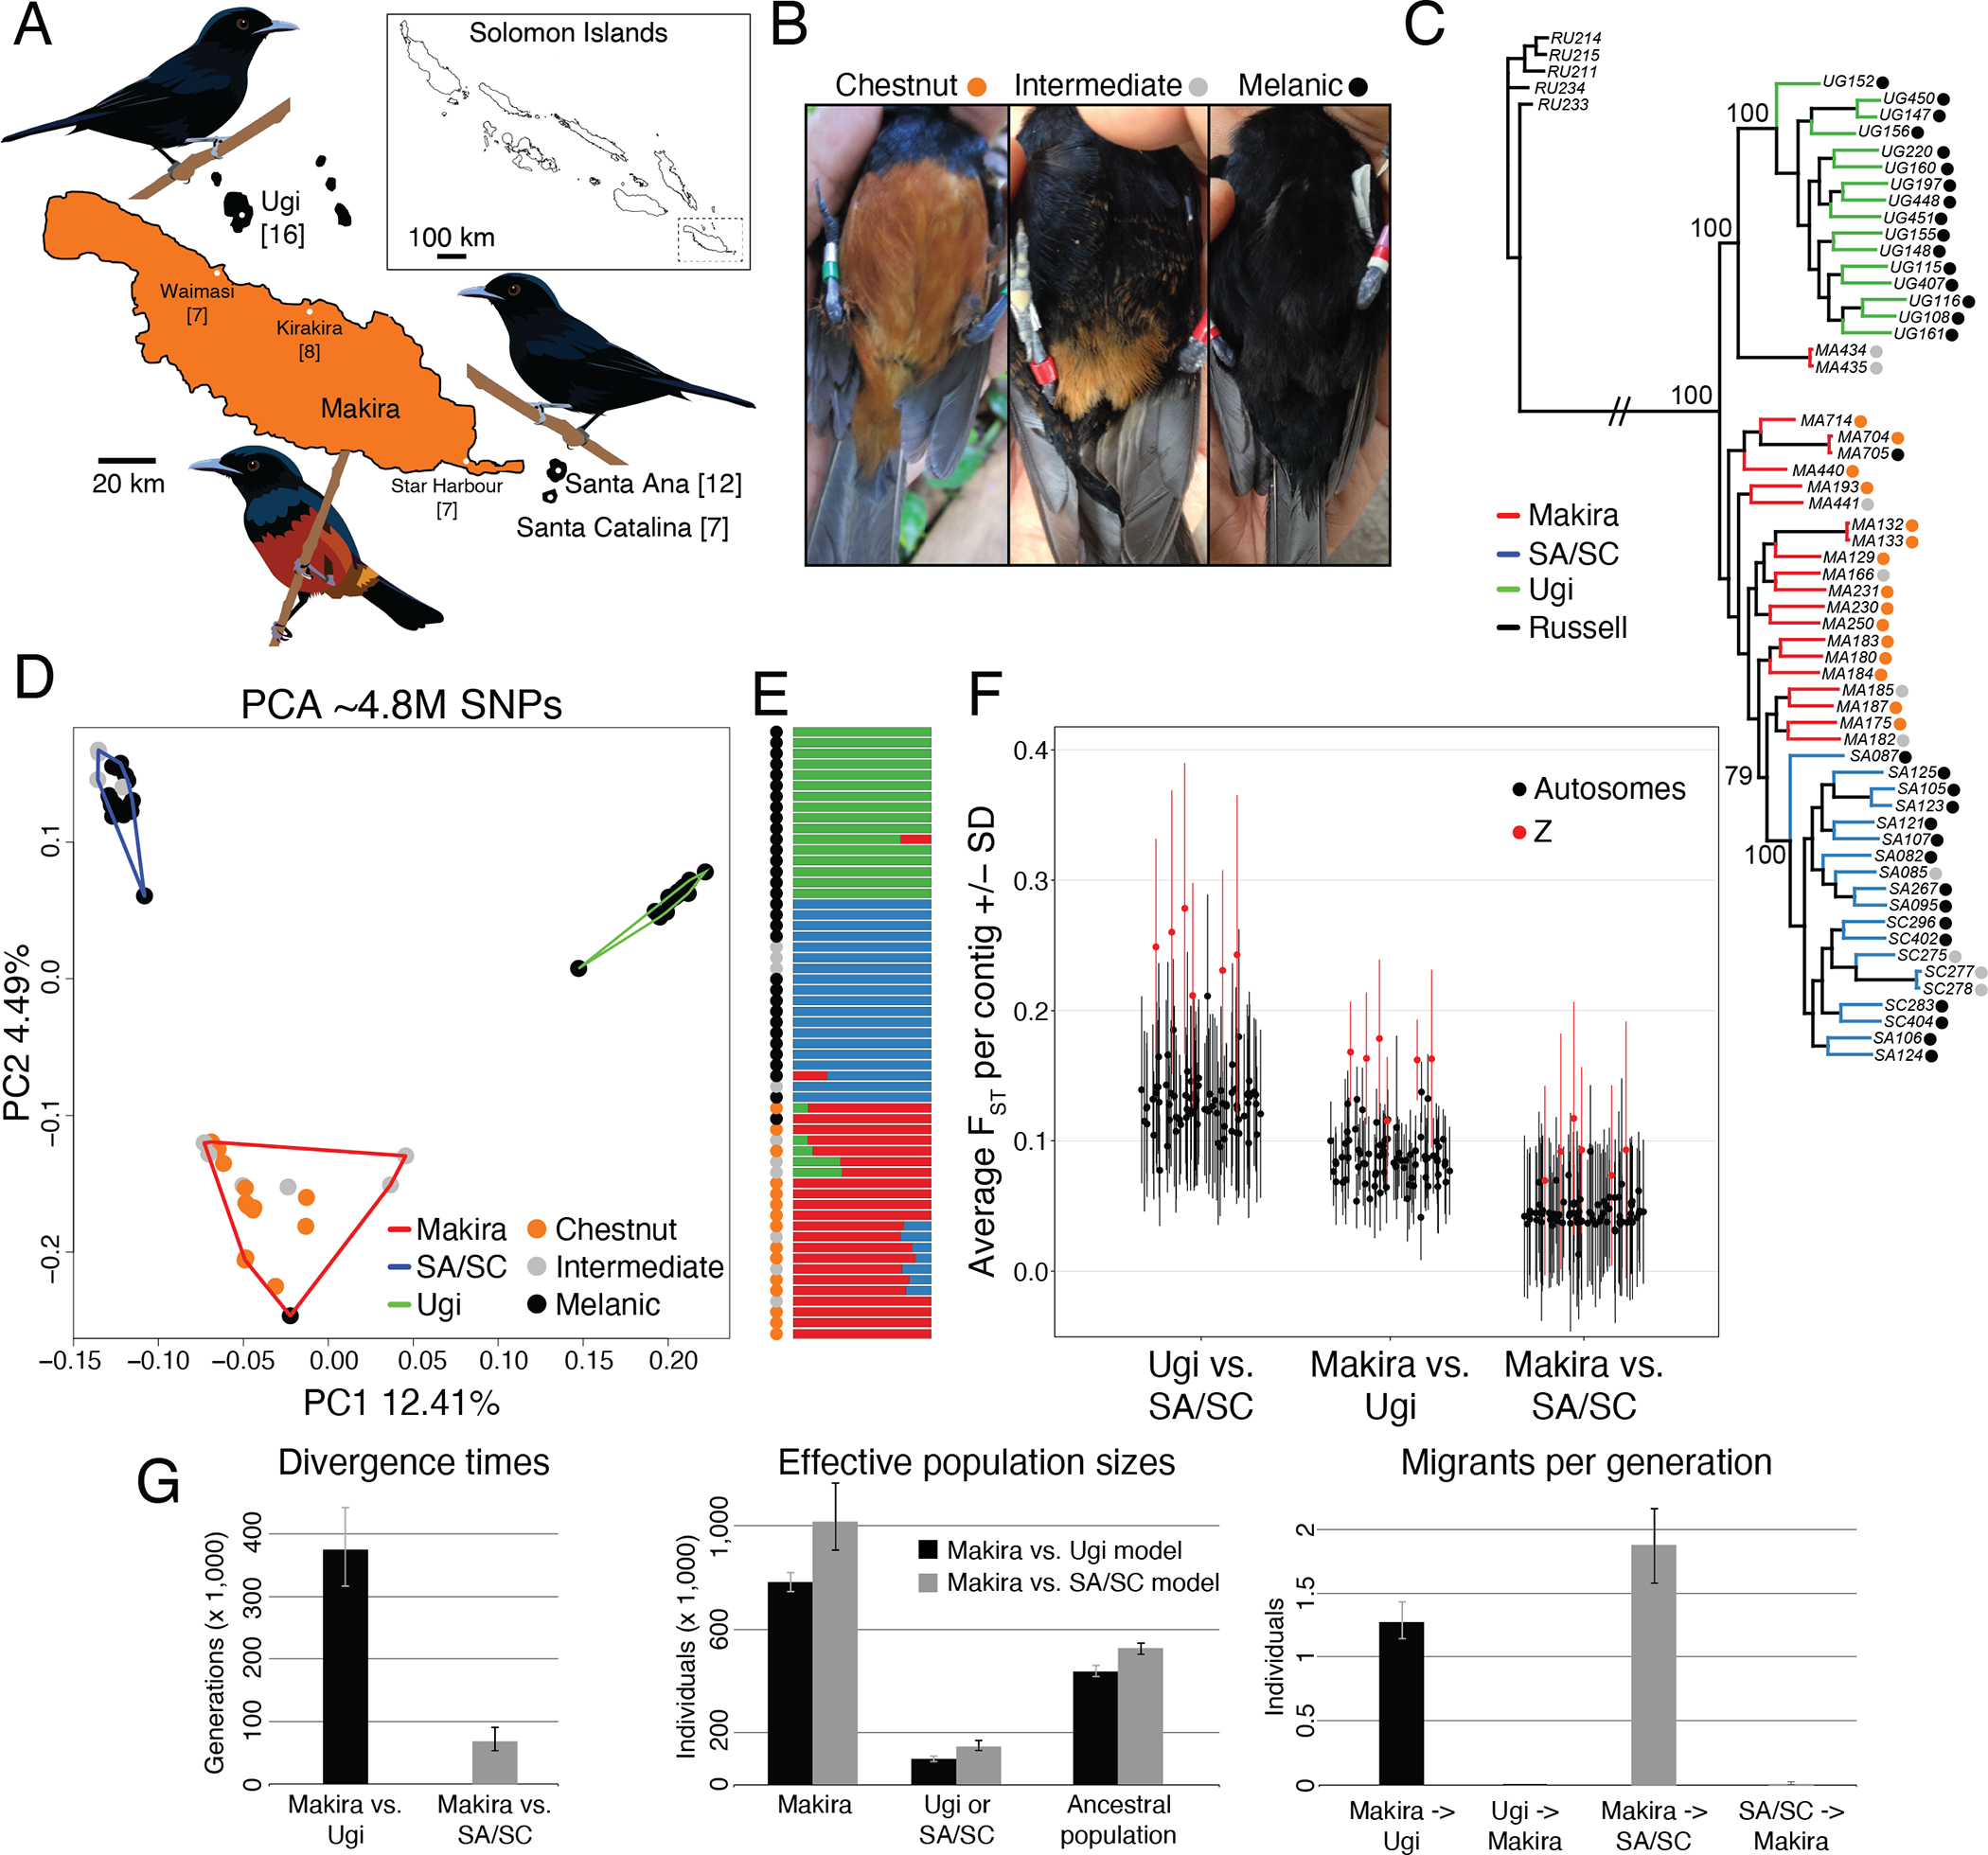
\includegraphics[width=\textwidth]{monarcha_figs/mon_F1.PNG}
    \caption[Genetic differentiation and demography of \textit{M. c. megarhynchus} and \textit{M. c. ugiensis}.]{\textbf{Genetic differentiation and demography of \textit{M. c. megarhynchus} and \textit{M. c. ugiensis}.} \textbf{A.} Study area, sample sizes and predominant phenotype on each island. The map was downloaded and modified from \href{www.diva-gis.org}{www.diva-gis.org}. \textbf{B.} Representative pictures of chestnut-bellied, intermediate and melanic individuals (color key used throughout Chapter \ref{chapter3}). Maximum Likelihood tree (\textbf{C}) and \acs{PCA} (\textbf{D}) indicating the origin and coloration phenotype of each individual. \textbf{E.} Admixture plot showing the proportion of ancestry for each individual belonging to three different genetic clusters. Each cluster is color-coded by the island from which samples originated and the phenotype is shown by color-coded circles on the left of the plot. \textbf{F.} Pairwise $F_{\mathrm{ST}}$ estimates summarized by contig. \textbf{G.} Demographic reconstructions indicating estimates of divergence times, effective population sizes, and migrants per generation.}
    \label{fig:mon-F1}
\end{figure}

Here we generate a reference genome for the Chestnut-bellied Monarch and obtain high coverage whole-genome data for a sample of individuals from Makira and its satellite islands. Our study aims to uncover the molecular targets and evolutionary forces that shape convergent evolution of adaptive traits that can contribute to generating prezygotic reproductive isolation. We use these data to quantify differentiation, reconstruct phylogenetic affinities, and infer the demographic history of these populations. We then use a genome-wide approach to identify variants associated with melanic plumage. Finally, we infer the evolutionary processes that have shaped these phenotypes on each of the satellite islands of Ugi and \ac{SA/SC}, estimate when mutations arose and the timing of these selective events.

\section{Results}

\subsection{Melanic populations are independently derived from a chestnut-bellied ancestor}
Birds grouped together by island, irrespective of their coloration phenotype (Fig. \ref{fig:mon-F1}C\&D). Individuals from the satellite islands of \ac{SA/SC} (which are primarily melanic, yet show a low prevalence of the intermediate coloration phenotype) and Ugi (which are exclusively melanic) formed island-specific clades which were embedded among clades containing primarily chestnut-bellied individuals from the larger island of Makira (Fig. \ref{fig:mon-F1}C). The relationships among birds from the three islands could not be resolved using mtDNA, as individuals from every locality share haplotypes (Fig. \href{https://journals.plos.org/PLOSGENETICS/article?id=10.1371/journal.pgen.1010474#sec017}{S1 online}). Consequently, melanism on the two satellite islands likely originated twice, independently from a chestnut-bellied ancestor (\cite{uy2016mutations,cooper2017genomic}). We did not observe clear evidence of early generation inter-island hybrids in the genome-wide \acs{PCA} (Fig. \ref{fig:mon-F1}D), however the two individuals from Makira which form a clade with the individuals from Ugi (Fig. \ref{fig:mon-F1}C) showed intermediate coloration and were sampled in the locality which is closest to Ugi (Waimasi), suggesting the possibility of either incomplete lineage sorting or gene flow. Furthermore, we observed Makira ancestry in one individual of each of the satellite islands, and \ac{SA/SC} or Ugi ancestry in a few individuals on Makira (Fig. \ref{fig:mon-F1}E). The admixed individuals on Makira were from the localities closest to the satellite island with which they shared ancestry (Waimasi for Ugi and Star Harbour for \ac{SA/SC}). The levels of differentiation among populations were largest between Ugi and \ac{SA/SC}, intermediate between Ugi and Makira, and smallest between \ac{SA/SC} and Makira (Fig. \ref{fig:mon-F1}F). The contigs showing the highest differentiation for each pairwise population comparison were in all cases Z-linked. The difference in the magnitude of genetic differentiation between populations could be due to variation in a combination of demographic parameters (i.e, the splitting time, the degree of gene flow experienced after this split, or the intensity of genetic drift due to differences in effective population sizes). We therefore used sequence data to conduct a demographic reconstruction with G-PhoCS, which suggested that the main reason for the observed difference in the levels of differentiation between populations was that Ugi split from Makira approximately six times earlier than \ac{SA/SC} branched from Makira (Fig. \ref{fig:mon-F1}G). Additionally, the effect of genetic drift is likely to be slightly stronger in Ugi, as its effective population size was inferred to be nearly two thirds of that of \ac{SA/SC} (and approximately one eighth of Makira’s). Finally, G-PhoCS inferred significant levels of gene flow from Makira into each of the satellite islands (higher into \ac{SA/SC}) and not in the reverse direction Fig. \ref{fig:mon-F1}G, suggesting that the admixture observed on Makira (Fig. \ref{fig:mon-F1}E) may be due to the retention of ancestral polymorphisms in this larger population.

\subsection{Melanism on each satellite island associates with mutations in different genes}
To test if the convergent melanic phenotype on each of the satellite islands was also convergent at the molecular level, we conducted two  genome wide association studies while controlling for population structure by including an inter-individual relatedness matrix as a covariate. The first included individuals from Makira and \ac{SA/SC} and revealed a single peak on contig 400 (corresponding to chromosome 11) composed of 61 \acsp{SNP} with association values above the significance threshold (Fig. \ref{fig:mon-F2}A). This region contained 15 annotated genes, including the coloration gene \textit{MC1R} (Fig. \ref{fig:mon-F2}B and \href{https://journals.plos.org/PLOSGENETICS/article?id=10.1371/journal.pgen.1010474#sec017}{S1 Table}). The second \acs{GWAS}, derived from individuals from Ugi and Makira showed seven association peaks with 83 annotated genes (Fig. \ref{fig:mon-F2}C and \href{https://journals.plos.org/PLOSGENETICS/article?id=10.1371/journal.pgen.1010474#sec017}{S1 Table}), suggesting a larger number of genes could mediate melanism on Ugi. One of these association peaks, on contig 947 (located on chromosome 20), contained four of the six strongest hits in the \acs{GWAS}. The \textit{MC1R} antagonist \textit{ASIP} was one of the 14 genes in this region (Fig. \ref{fig:mon-F2}D). The variants within the seven association peaks were in high \ac{LD} (average intrachromosomal $R^2 = 0.84$; average interchromosomal $R^2 = 0.79$; Fig. \href{https://journals.plos.org/PLOSGENETICS/article?id=10.1371/journal.pgen.1010474#sec017}{S2 online}). We did not find other known coloration genes within the remaining association peaks (\href{https://journals.plos.org/PLOSGENETICS/article?id=10.1371/journal.pgen.1010474#sec017}{S1 Table}), suggesting these genes have unknown functions in melanism or mediate other differences between the Ugi and Makira populations which may covary with changes in coloration (e.g., Ugi individuals are larger than those from Makira). Three of the seven association peaks were on the Z sex chromosome, which is consistent with this chromosome evolving faster than the autosomes in birds (\cite{irwin2018sex}). Additionally, when comparing within the region encompassed by the association peaks containing \textit{MC1R} and \textit{ASIP} and outside of this region (for contig 400 and 947 separately), we observed higher levels of differentiation between Makira and each of the satellite islands (Fig. \href{https://journals.plos.org/PLOSGENETICS/article?id=10.1371/journal.pgen.1010474#sec017}{S3A\&B online}).

\begin{figure}%[h]
    \centering
    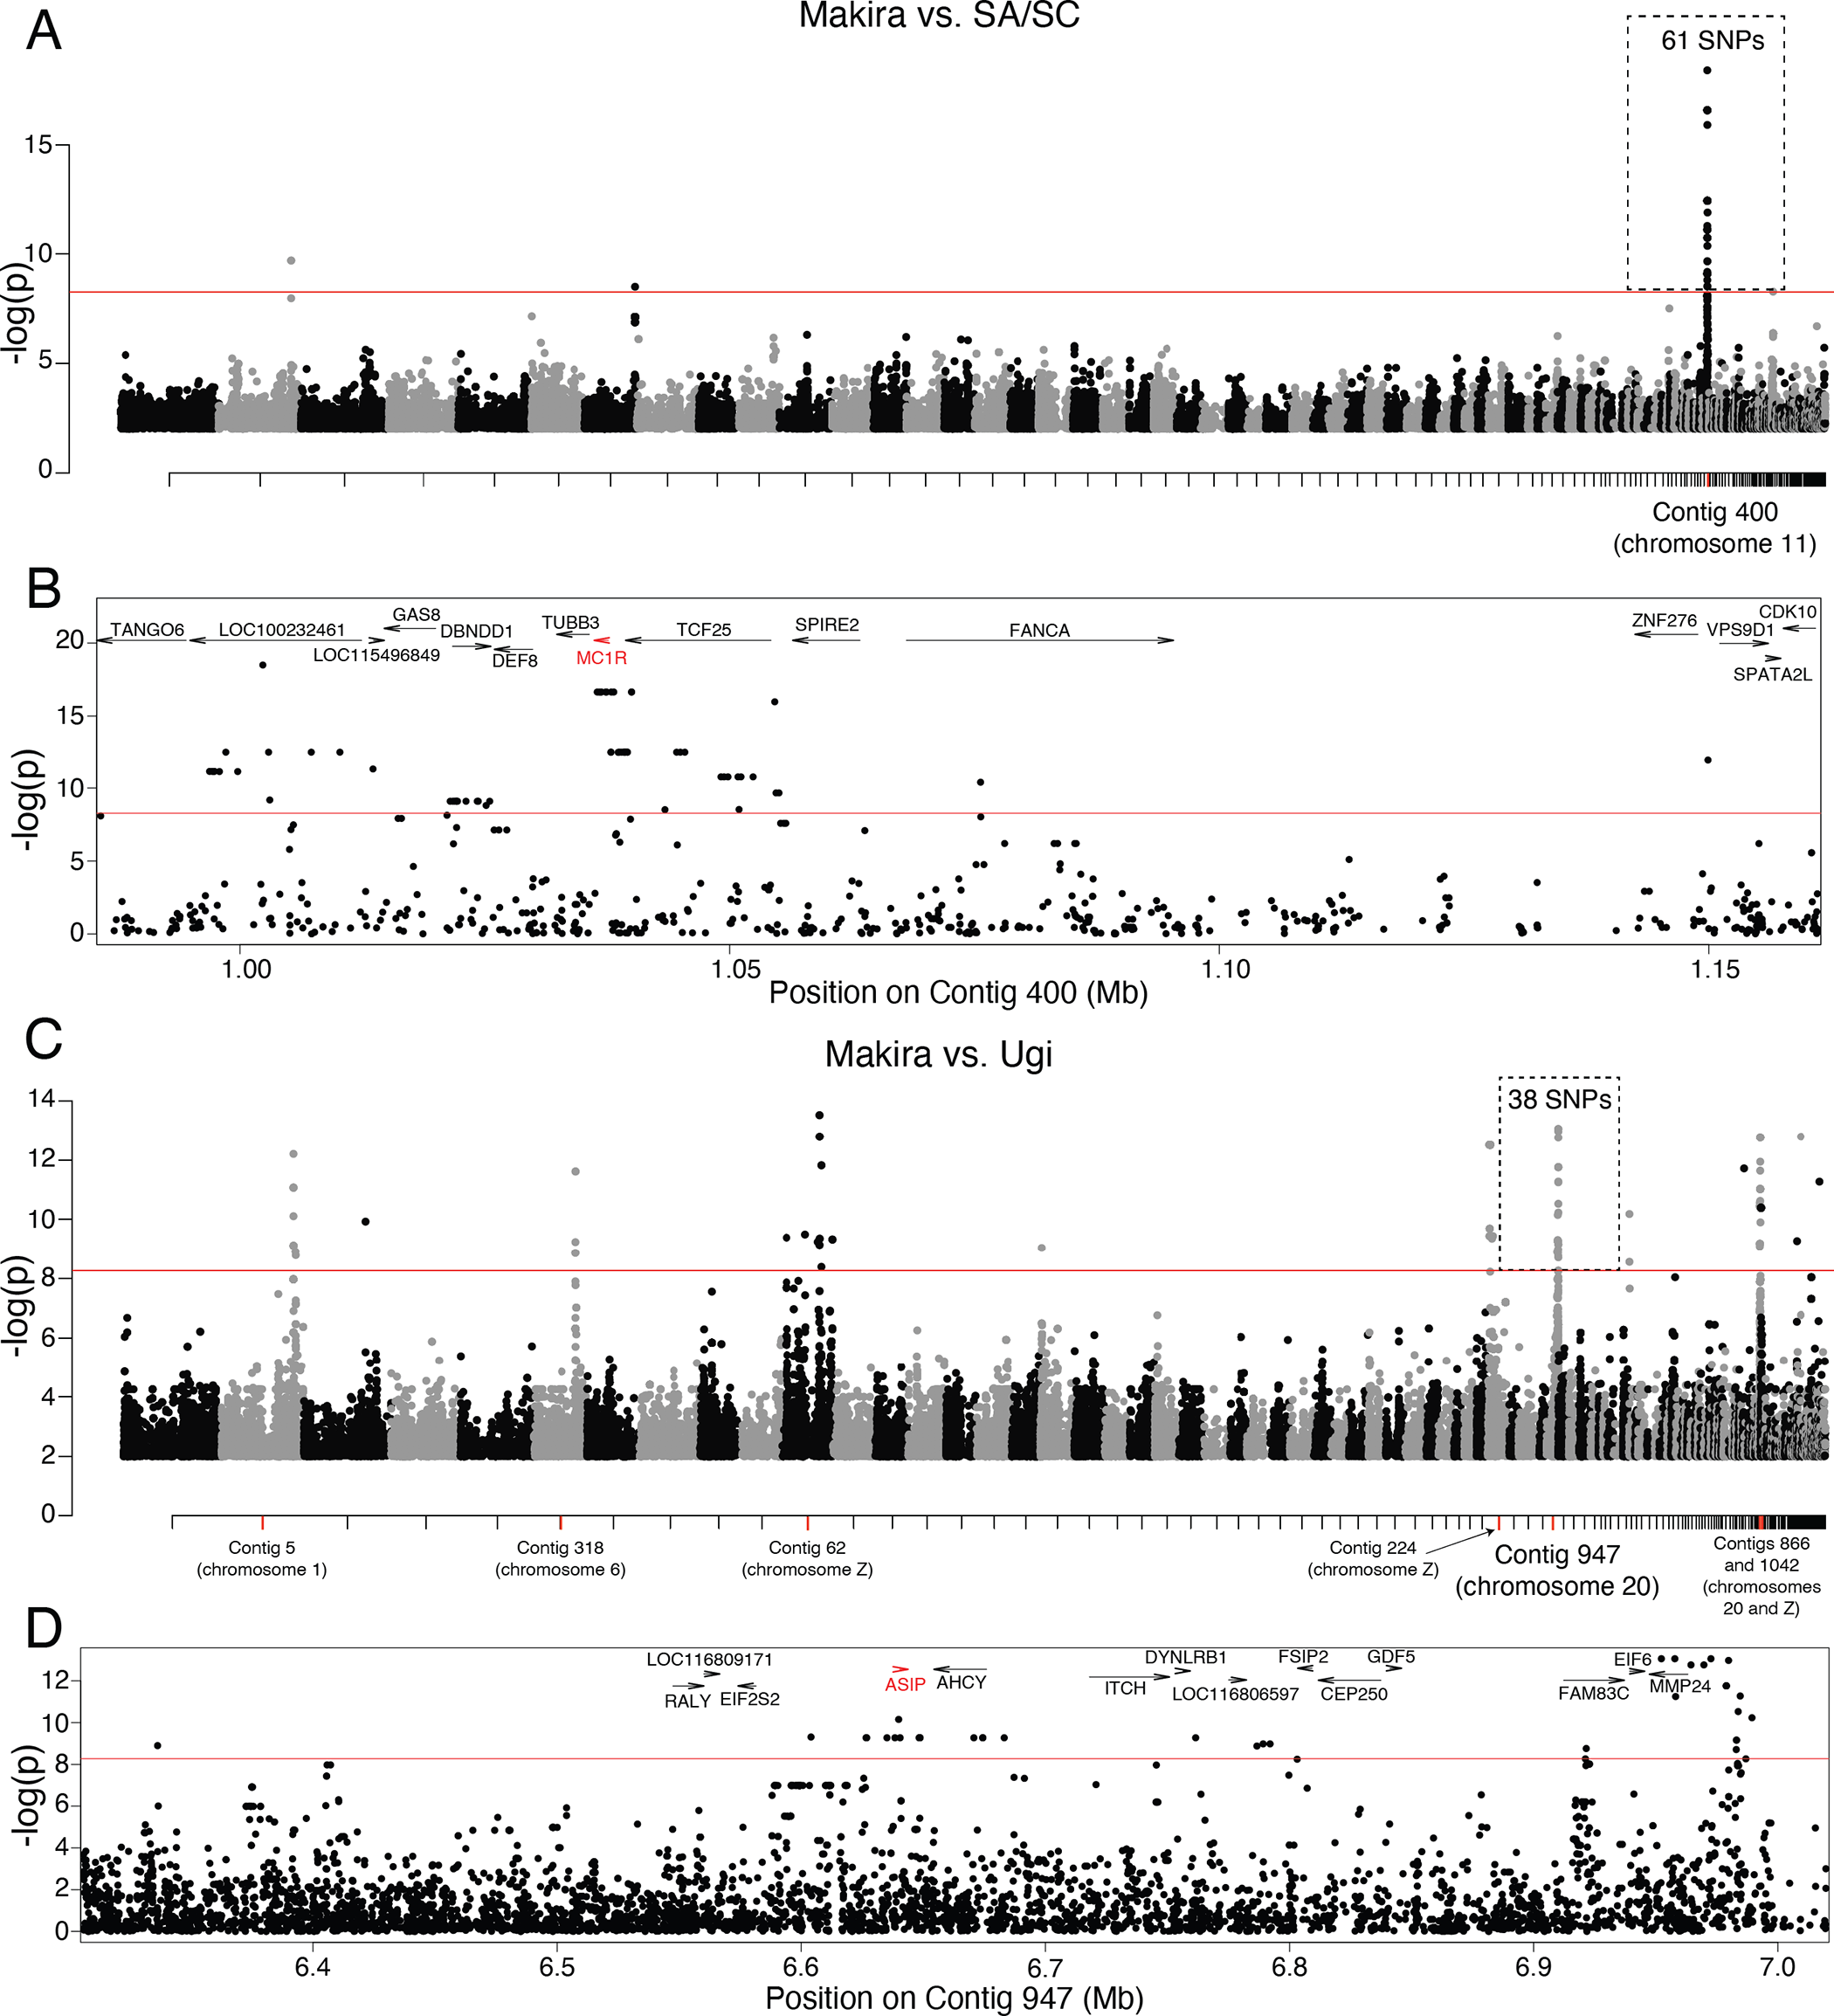
\includegraphics[width=\textwidth]{monarcha_figs/mon_F2.PNG}
    \caption[Genome wide association study comparing individuals from subspecies of \textit{Monarcha castaneiventris}.]{\textbf{Genome wide association study comparing individuals from subspecies of \textit{Monarcha castaneiventris}.} \textbf{A.} Manhattan plot obtained from the \acs{GWAS} comparing individuals from Makira and \ac{SA/SC}. \textbf{B.} Zoom-in to the association peak in \textbf{A} indicating gene annotations within this region with \textit{MC1R} in red. Equivalent plots for the \acs{GWAS} obtained with individuals from Makira and Ugi (\textbf{C}, \textbf{D}).}
    \label{fig:mon-F2}
\end{figure}

The melanic individuals from \ac{SA/SC} had two haplotypes in the region which contained the 61 association hits on contig 400, which were different from the most prevalent haplotype on Makira and Ugi (Figs. \href{https://journals.plos.org/PLOSGENETICS/article?id=10.1371/journal.pgen.1010474#sec017}{S4 and S5 online}). Three variants fell within the coding region of \textit{MC1R}; two of these positions involved synonymous changes and one coded for an \textit{Asp119Asn} substitution. Similarly, all the individuals from Ugi possessed two haplotypes that were different from the main one present in \ac{SA/SC} and Makira individuals in the association region around \textit{ASIP} (38 \acsp{SNP}; Figs. \href{https://journals.plos.org/PLOSGENETICS/article?id=10.1371/journal.pgen.1010474#sec017}{S5 and S6 online}). A single position fell within the coding region of \textit{ASIP} and involved a non-synonymous \textit{Ile55Thr} substitution, with all Ugi individuals carrying the \textit{Thr55} allele. In conclusion, melanic individuals always carried two copies of the coding \textit{MC1R} mutation (\textit{Asn119}) observed on \ac{SA/SC} or of the coding \textit{ASIP} mutation (\textit{Thr55}) observed on Ugi.

\subsection{The regions of the genome containing \textit{MC1R} and \textit{ASIP} show signatures of selective sweeps}
We first searched for signatures of selection by calculating summary statistics from the focal contigs containing coloration genes. The region which includes the \textit{MC1R} gene produced negative values of Tajima’s $D$ and low nucleotide diversity in the \ac{SA/SC} population (Fig. \ref{fig:mon-F3}A), as expected for a selective sweep, and high H12 and intermediate H2/H1 values, which are consistent with a relatively soft selective sweep (Fig. \ref{fig:mon-F3}B). However, because of the windowed nature of this analysis we are cautious in interpreting the specific type of sweep that affected the \textit{MC1R} gene. We observed windows within the peak on contig 947 for the Ugi population that showed an overall similar pattern to the one seen for \textit{MC1R} on \ac{SA/SC} (Fig. \ref{fig:mon-F3}C\&D). The positive value of Tajima’s $D$ for the window containing \textit{ASIP} on contig 947 (1.4) may be consistent with balancing selection, yet represents an average for a 5 kb window which only included a single \acs{SNP} (out of 12) from the gene region. In fact, when we calculate Tajima’s $D$ for 500 bp windows, the one which includes \textit{ASIP} has a value close to zero (0.25; calculated from 3 \acsp{SNP} in that window). We opted to present our results for 5 kb windows as these contain an average of 25 \acsp{SNP} per window (vs. an average of 3 \acsp{SNP} for 500 bp windows) and therefore represent more robust values of the summary statistics. Finally, we note that genome-wide values of Tajima’s $D$ tend to be close to zero for the three populations (-0.6 for Makira and 0.1 for both \ac{SA/SC} and Ugi), which suggests this statistic hasn’t been strongly impacted by demographic trends.

\begin{figure}[h]
    \centering
    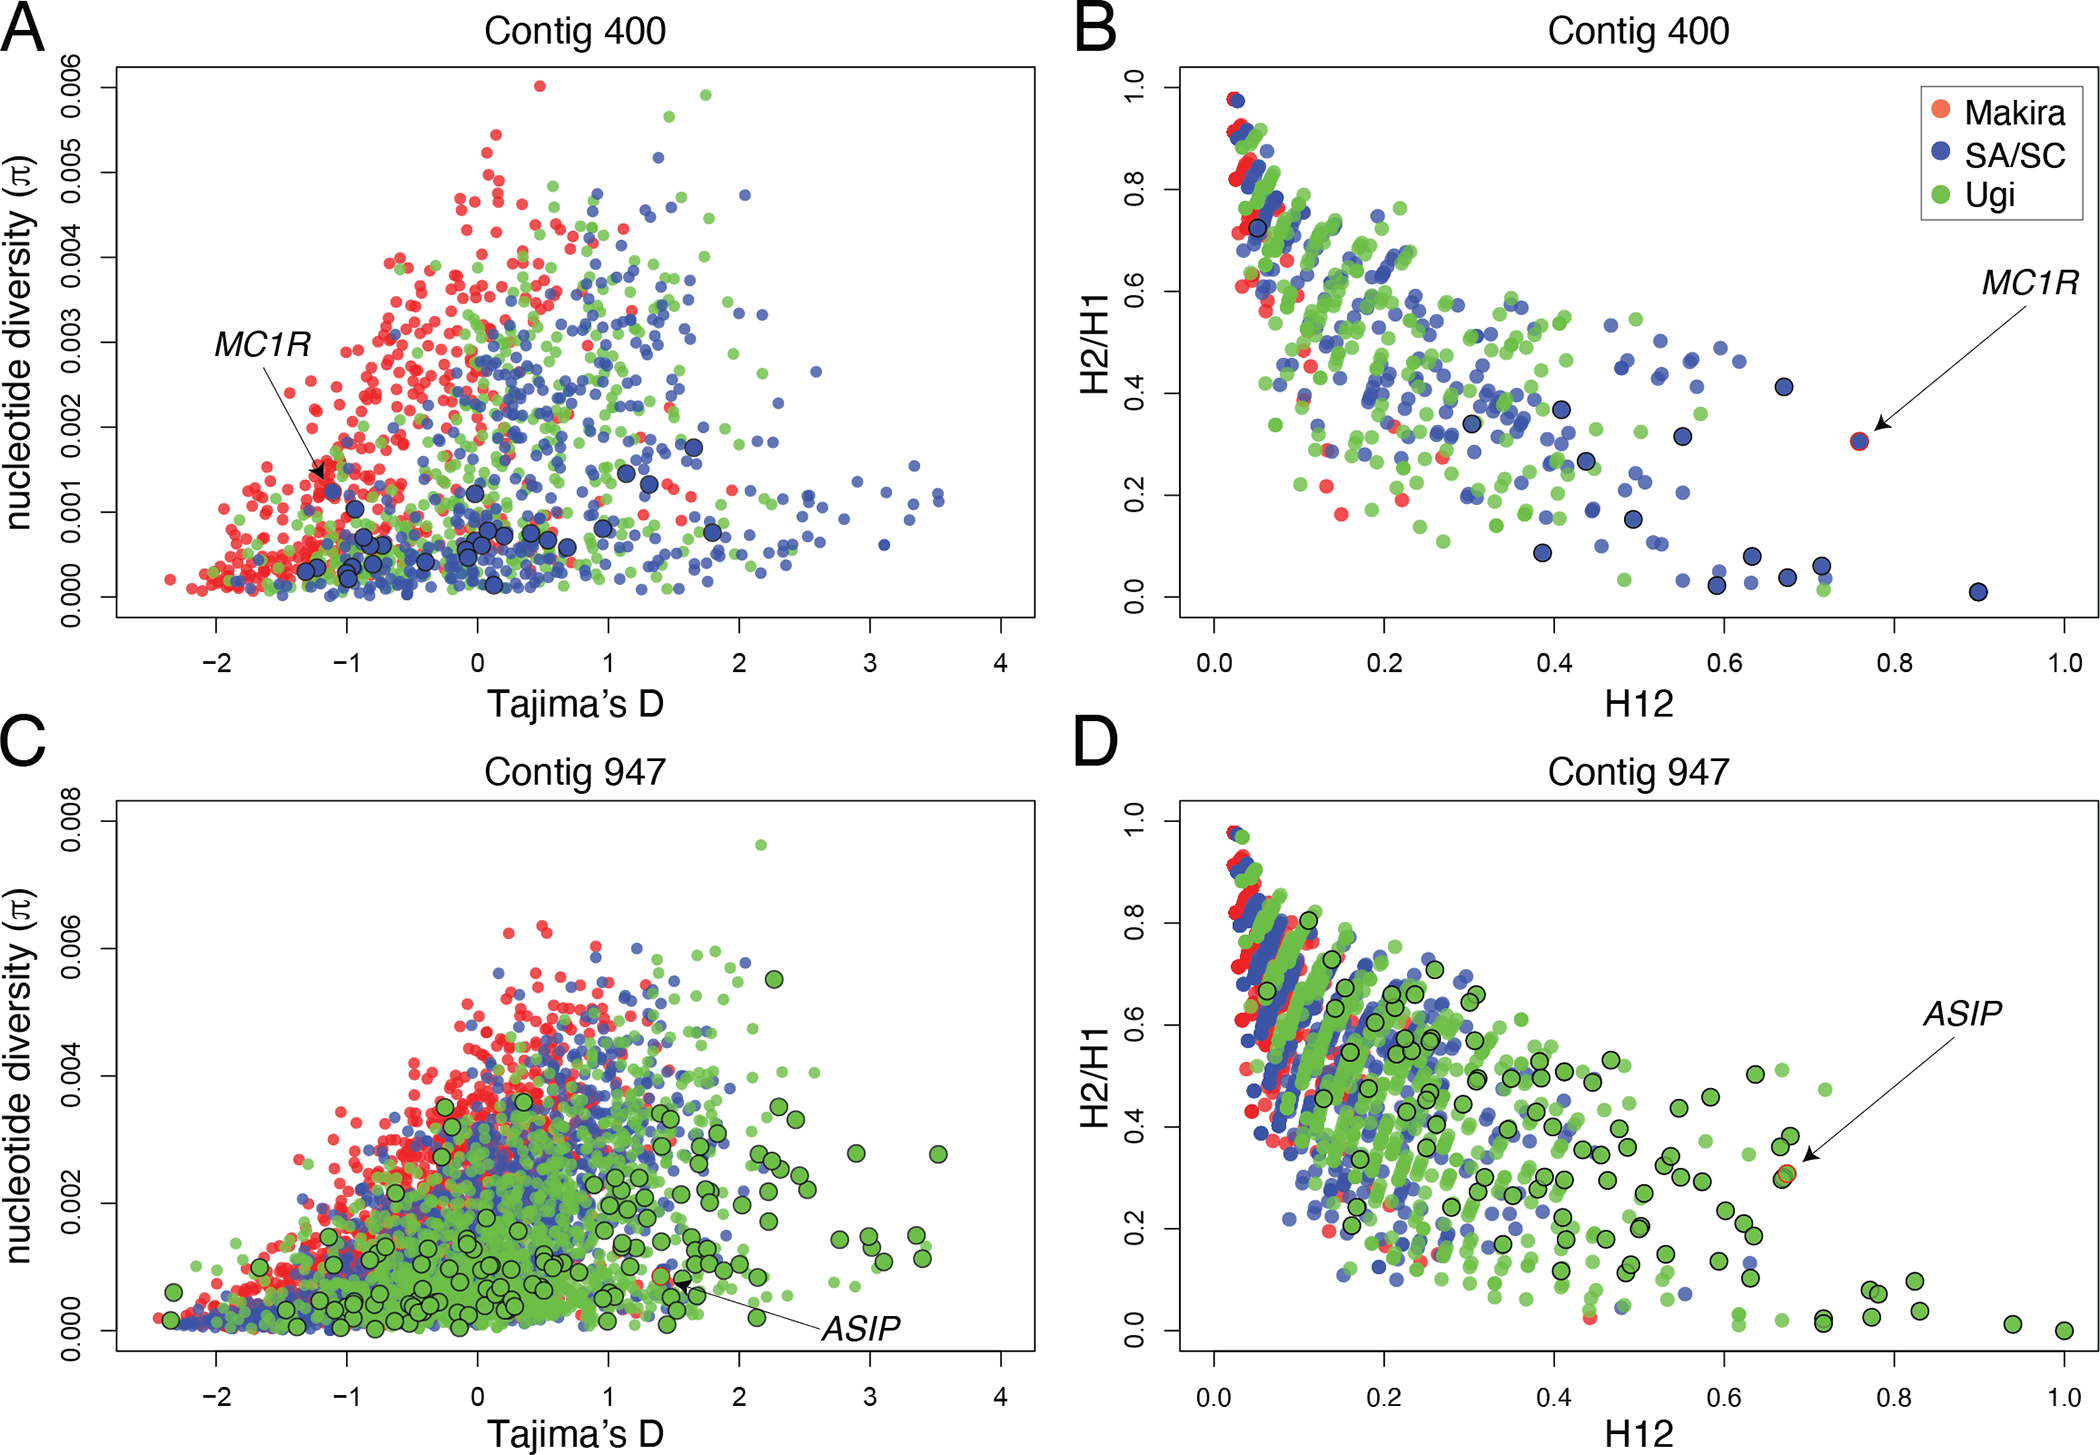
\includegraphics[width=\textwidth]{monarcha_figs/mon_F3.PNG}
    \caption[Evidence of a selective sweep in \textit{MC1R} for the \ac{SA/SC} population and on \textit{ASIP} in the Ugi population.]{\textbf{Evidence of a selective sweep in \textit{MC1R} for the \ac{SA/SC} population and on \textit{ASIP} in the Ugi population.} Biplots of Tajima’s $D$ vs. nucleotide diversity for contig 400 and contig 947 (\textbf{A}, \textbf{C}). Biplots of H12 vs. H2/H1 for the same contigs as above (\textbf{B}, \textbf{D}). Dots represent statistics derived from 5 kb windows (Tajima’s $D$ vs. nucleotide diversity) or 100-\acs{SNP} windows (H12 vs. H2/H1), and are color coded based on the population of origin. Larger dots denote windows that belong to the outlier peak region, and those that have a red outline include the focal gene indicated by the arrow.}
    \label{fig:mon-F3}
\end{figure}

\section{Discussion}

\section{Materials and methods}

\section{Supplementary material}
Supporting information is available at \href{https://journals.plos.org/PLOSGENETICS/article?id=10.1371/journal.pgen.1010474#sec017}{\textit{PLoS Genetics} online}. The computer code for this project has been deposited in GitHub repos, \href{https://github.com/CshlSiepelLab/bird_capuchino_analysis}{\texttt{bird\_capuchino\_analysis}} and \href{https://github.com/CshlSiepelLab/arg-selection}{\texttt{arg-selection}}. Genomic data have been archived in GenBank (BioProject ID PRJNA835722).